\FloatBarrier
\section{Liaison Ethernet : les couches 1 et 2}
\subsection{Couche 1 : Transmission de données}
Pour la couche 0, la norme Ethernet définit les supports physiques possibles. En fonction de la norme suivie, différents débits
\begin{description}
  \item [10 BaseT : ] Paire torsadée \SI{100}{Mbit/s}
  \item [100 BaseT : ] Paire torsadée \SI{100}{Mbit/s}
  \item [1000 BaseT : ] Paire torsadée \SI{1}{Gbit/s}
  \item [1000 BaseX : ] Paire torsadée \SI{1}{Gbit/s}
  \item [Wifi] Liaison hertzienne \SI{54}{Mbit/s} à \SI{433}{Mbit/s}
\end{description}

Le format de la norme est également défini par la norme Ethernet. Par exemple, la norme 10 Bast-TX utilise le codage Manchester pour transmettre les données ainsi que l'horloge sur une seule paire de câble. La détection d'un 1 ou d'un 0 se fait alors en fonction du sens du front (montant ou descandante) et non du niveau sur un front d'horloge (voir Figure~\ref{fig:manchesterCode}).

\begin{figure}[h]
  \centering
  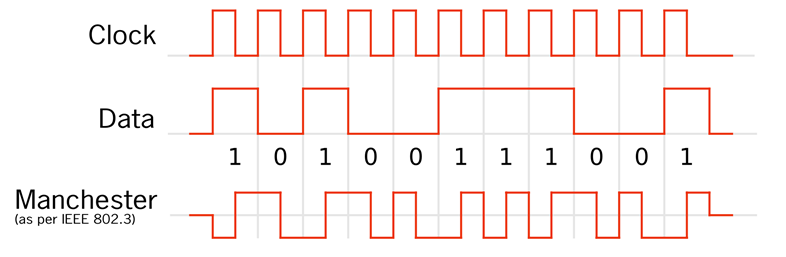
\includegraphics[width=.7\textwidth]{../../images/materiel/manchesterCode}
  \caption{Codage Manchester : L'horloge et les données sont envoyées sur le même signal}
  \label{fig:manchesterCode}
\end{figure}

\subsection{Couche 2 : Trame Ethernet}
\subsubsection{L'adresse MAC}
Comme discuté en section \ref{sec:CarteReseau}, chaque organe connecté au réseau possède une adresse MAC \textbf{unique} dans le monde. Chaque constructeur de carte réseau a un préfixe qui lui est attribué, puis il attribue à chaque matériel qu'il produit un code unique. Ainsi, théoriquement, tous les appareils connectés au réseaux possèdent une adresse MAC différente. On représente généralement une adresse MAC sous la forme hexadécimale pour des raisons évidentes de lisibilités. Par exemple, l'adresse MAC 00:1B:44:11:3A:B7 est décomposée dans le Tableau~\ref{tab:macExample}. Il est possible de retrouver le fabriquant d'une carte réseau via de nombreux site comme \url{https://macvendors.com/}.

\begin{table}[h!t]
\centering
  \begin{tabular}{ccc|ccc}
    octet 1 & octet 2 & octet 3 & octet 4 & octet 5 & octet 6\\
    \hline
    00      & 1B    &     44    & 11      &3A       &B7\\\hline
    \multicolumn{3}{c|}{Constructeur : }&\multicolumn{3}{c}{identifiant unique}\\
    \multicolumn{3}{c|}{SanDisk Corporation}&\multicolumn{3}{c}{}

  \end{tabular}
  \caption{Décomposition d'une adresse MAC : 00:1B:44:11:3A:B7}
  \label{tab:macExample}
\end{table}

\UPSTIaRetenir{L'adresse MAC est l'identifiant utilisé par le protocole Ethernet pour connaître le destinataire d'un message au sein d'un réseau.}
On peut faire une analogie entre l'adresse MAC et le nom que l'on écrirait sur une enveloppe pour la transmettre à une personne.

\begin{UPSTIactivite}
  Retrouver le constructeur de votre carte réseau à partir de son adresse MAC.
\end{UPSTIactivite}

\subsubsection{Décomposition d'une trame}

Lors de l'envoi d'une trame sur le réseau Ethernet, le premier niveau d'encapsulation correspond au protocole Ethernet. Dans un réseau local, c'est le protocole Ethernet qui définit le destinataire de la trame ainsi que son expéditeur. Tous deux sont identifiés par leur adresse MAC (adresse physique).
\begin{itemize}
  \item
\end{itemize}

\begin{description}
  \item [Préambule : ] Utilisation d’un modèle défini d’alternance de bits 1 et 0 pour synchroniser les appareils.
  \item [SFD : ]Délimitateur de début de Trame
  \item [MAC destination : ] Adresse de l'appareil destinataire
  \item [MAC expediteur : ] Adresse de l'appareil expediteur
  \item [Longueur/Type : ] Définit le type (ou parfois la longueur) de la trame.
  \begin{itemize}
    \item Dans le cas d'un envoi de trame TCP/IP, le type vaudra toujours \num{0x0800}
  \end{itemize}
  \item [Donnée encapuslées : ]Données à envoyer
  \item [CRC : ] La séquence de contrôle de trame contient une valeur de 4 octets créée par le périphérique qui envoie les données et recalculée par le périphérique de destination pour vérifier si les trames sont endommagées.
\end{description}

\UPSTIremarque{La taille d'une trame Ethernet doit être comprise entre 64 octets et 1564 octets. C'est pourquoi les données encapsulées ont une longueur allant de 46 à 1500 octets. Si on souhaite envoyer une trame plus courte, on ajoutera alors des données de bourrage (bits inutiles) pour atteindre la taille minimale.}

\begin{figure}
\centering
    \definecolor{Gray}{gray}{0.9}
\definecolor{Gray2}{gray}{0.7}
\newcolumntype{a}{>{\columncolor{Gray}}c}
\newcolumntype{b}{>{\columncolor{Gray2}}c}

\begin{tabular}{|a|a|a|a|a|a|a|a|c|c|c|c|c|c|c|c|c|c|c|c|c|c|b|b|b|b|b|b|b|b|b|b|b|a|a|a|a|}
\hline
  &&&&&&&&&&&&&&&&&&&&&&&&&&\multicolumn{3}{|b|}{\dots}&&&&&&&& \\\hline
  \multicolumn{7}{|a|}{}          & S &\multicolumn{6}{c|}{Adresse}               &\multicolumn{6}{c|}{Adresse}             & \multicolumn{2}{c|}{L}  &\multicolumn{11}{b|}{}     &\multicolumn{4}{a|}{C}  \\
  \multicolumn{7}{|a|}{Préambule} & F &\multicolumn{6}{c|}{MAC}                   &\multicolumn{6}{c|}{MAC}                 & \multicolumn{2}{c|}{/}  &\multicolumn{11}{b|}{Data}  &\multicolumn{4}{a|}{R}  \\
  \multicolumn{7}{|a|}{}          & D &\multicolumn{6}{c|}{\textbf{destinataire}} &\multicolumn{6}{c|}{\textbf{expediteur}} & \multicolumn{2}{c|}{T}  &\multicolumn{11}{b|}{}      & \multicolumn{4}{a|}{C}  \\\hline
  \multicolumn{7}{|a|}{7 octets}  & 1o &\multicolumn{6}{c|}{6 octets}             &\multicolumn{6}{c|}{6 octets}            & \multicolumn{2}{c|}{2o}  &\multicolumn{11}{b|}{De 46 à 1500 octets}      &\multicolumn{4}{a|}{4o}  \\\hline

\end{tabular}

  \caption{Décomposition d'une trame Ethernet}
\end{figure}

\subsubsection{Exemple d'envoi de trame : Concentrateur vs Commutateur}
\paragraph{Concentrateur}
Un concentrateur (souvent appelé hub) est un appareil appartenant à la couche 1 (physique, cf \ref{sec:couches}). Cela signifie que cet appareil n'a pas accès aux contenus des couches supérieures. Il est donc incapable d'identifier le destinataire d'un message.

Ainsi, lorsque l'on relie des appareil à l'aide d'un concentrateur (hub), les données envoyées sont transmises à tous les appareils connectés. Il appartiendra alors aux appareil de décider d'ouvrir ou non le message selon s'il leur est destiné ou non. La Figure~\ref{fig:trameConcentrateur} illustre l'envoi d'une trame par l'hôte H1 à l'hôte H6. Tous les appareils reçoivent la trame mais seul H6 l'ouvre car l'adresse MAC du message lui correspond. Cette animation est disponible à la section \href{https://static-course-assets.s3.amazonaws.com/NetEss/fr/index.html#3.4.1.3}{3.4.1.3} du cours netacad.

\UPSTIremarque{Puisque tous les appareils reçoivent la trame, l'utilisation d'un concentrateur peut être vue comme peu sécurisée. En effet, même s'il ne sont pas sensé l'ouvrir, n'importe quelle hôte pourrait avoir accès au message envoyé de H1 à H6.}



\paragraph{Commutateur}
Un commutateur (souvent appelé switch) est un appareil appartenant à la couche 2 (liaison, cf \ref{sec:couches}). Il a donc accès aux adresses MAC de la trame et est donc capable d'identifier le destinataire d'un message.

Ainsi, lorsque l'on relie des appareil à l'aide d'un commutateur (switch), ce dernier redirige le message uniquement vers son destinataire. La Figure~\ref{fig:trameCommutateur} illustre l'envoi d'une trame par l'hôte H1 à l'hôte H6. Puisqu'il connaît l'identité (adresse MAC) des hôtes connecté, le commutateur ne transmet le message que sur le câble connecté à H6. Cette animation est disponible à la section \href{https://static-course-assets.s3.amazonaws.com/NetEss/fr/index.html#3.4.2.1}{3.4.2.1} du cours netacad.

\UPSTIremarque{L'utilisation d'un switch (commutateur) présente deux avantages majeurs : \begin{itemize}
  \item Le réseau est moins encombré puisque les messages ne transitent pas inutilement vers des hôtes auxquels ils ne sont pas destinés.
  \item Il est \textit{a-priori} impossible pour les autres hôtes de lire le message puisque celui-ci n'arrive pas jusqu'à eux.
\end{itemize}}

\UPSTIremarque{L'étude de la table MAC d'un commutateur fait l'objet d'un exercice de TD.}

\begin{figure}[p]
\centering
\begin{subfigure}{\textwidth}
\centering
  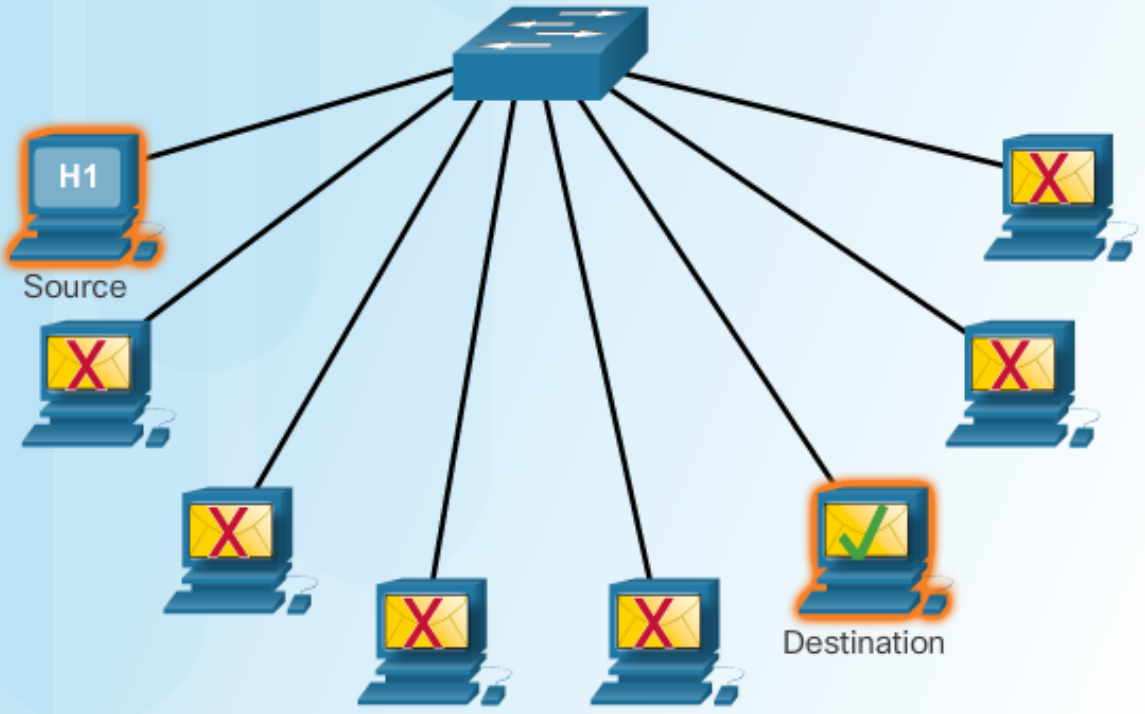
\includegraphics[width=.7\linewidth]{images/ethernet/concentrateurCroped}
  \caption{Envoi d'une trame par un concentrateur. Le message est transmis à tous les appreils connectés.}
  \label{fig:trameConcentrateur}
\end{subfigure}

\vspace{1cm}

  \begin{subfigure}{\textwidth}
  \centering
  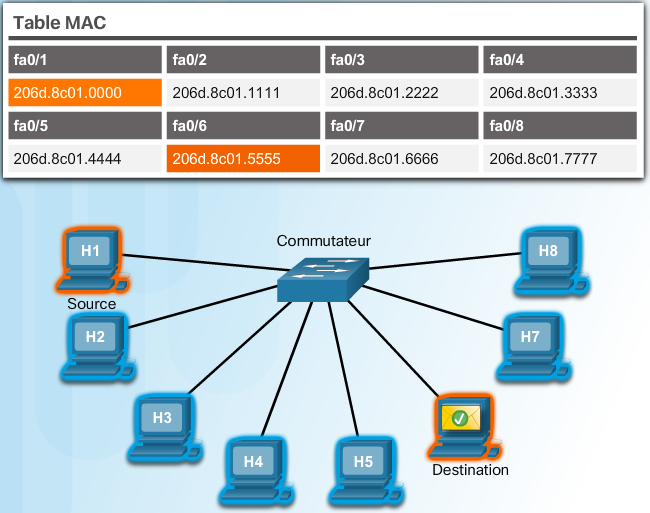
\includegraphics[width=.7\linewidth]{images/ethernet/communtateur}
  \caption{Envoi d'une trame par un commutateur. Le message est transmis uniquement à son destinataire.}
  \label{fig:trameCommutateur}
  \end{subfigure}
  \caption{Concentrateur vs Commutateur}
\end{figure}
